\documentclass[twoside,twocolumn]{article}

\usepackage{blindtext} 
\usepackage{graphicx}
\usepackage[sc]{mathpazo} 
\usepackage[T1]{fontenc} 
\linespread{1.05} 
\usepackage{microtype} 

\usepackage[utf8]{inputenc}
\usepackage[spanish,english]{babel} 

\usepackage[hmarginratio=1:1,top=32mm,columnsep=20pt]{geometry} 
\usepackage[hang, small,labelfont=bf,up,textfont=it,up]{caption} 
\usepackage{booktabs} 
\usepackage{lettrine} 
\usepackage[table,xcdraw]{xcolor}
\usepackage{multicol, blindtext}

\usepackage{enumitem} 
\setlist[itemize]{noitemsep} 


\usepackage{abstract} 
\renewcommand{\abstractnamefont}{\normalfont\bfseries} 
\renewcommand{\abstracttextfont}{\normalfont\small\itshape} 


\usepackage{titlesec} 
\renewcommand\thesection{\Roman{section}} % 
\renewcommand\thesubsection{\roman{subsection}} 
\titleformat{\section}[block]{\large\scshape\centering}{\thesection.}{1em}{} 
\titleformat{\subsection}[block]{\large}{\thesubsection.}{1em}{} 


\usepackage{fancyhdr} 
\pagestyle{fancy} 
\fancyhead{} 
\fancyfoot{} 
\fancyhead[C]{Frameworks de pruebas $\bullet$ Diciembre 2020 $\bullet$ } 
\fancyfoot[RO,LE]{\thepage} 


\usepackage{titling}
\usepackage{hyperref} 
\usepackage{listings}
\usepackage{xcolor}

\lstset{
  basicstyle=\ttfamily,
  columns=fullflexible,
  frame=single,
  breaklines=true,
  postbreak=\mbox{\textcolor{red}{$\hookrightarrow$}\space},
}

%----------------------------------------------------------------------------------------
%	TILULOS
%----------------------------------------------------------------------------------------


\setlength{\droptitle}{-4\baselineskip} 

\pretitle{\begin{center}\Huge\bfseries} 
\posttitle{\end{center}} 
\title{Frameworks de pruebas} 
\author{Percy Taquila Carazas, Katerin Merino Quispe, Abraham Lipa Calabilla,
\\Edwart Balcon Coahila, Lisbeth Espinoza Caso}
\date{\today} 
\renewcommand{\maketitlehookd}{

\selectlanguage{english}
\begin{abstract}
\noindent 
In this article we will see how important tests can be, showing different causes of software failures.
Also the development of each Test Frameworks named in this article.

\end{abstract}


\selectlanguage{spanish}
\begin{abstract}
\noindent 

En este articulo veremos lo importante que pueden llegar a ser las pruebas, mostrando diferentes causas de fallas en el software.
Tambien el desarrollo de cada Frameworks de Pruebas nombrado en este articulo.

\end{abstract}

}

%----------------------------------------------------------------------------------------

\begin{document}

% Print the title
\maketitle

%----------------------------------------------------------------------------------------
%	INTRODUCCION
%----------------------------------------------------------------------------------------

\section{Introduccion}


\lettrine[nindent=0em,lines=3]{L}a arquitectura de los microservicios tiene una estructura modular en la que, en lugar de conectar componentes, el software se divide en componentes. Las aplicaciones, por lo tanto, se construyen como un conjunto de servicios que son desplegados de forma independiente, escalables y flexibles.

Las aplicaciones de Internet utilizan API de servicios web en forma de SOAP (Simple Object Access Protocol) o REST (Representational State Transfer). Aunque hay diferencias técnicas y de arquitectira, en términos de entrada-salida, ambos protocolos utilizan formato basados en texto; SOAP utiliza la notación XML y REST utiliza la notación JSON. Ambos formatos son fáciles de aprender.

Aunque los Microservicios ofrecen muchos beneficios, como escalabilidad, modificabilidad y agilidad en la entrega continua, utilizando microservicios, hacemos que las pruebas de software sean más complejas. Al testear microservicios, debemos asegurarnos no sólo que el microservicio específico funcione, sino también que todos sus microservicios, cuando están juntos, se comporten como se esperaba. Para ellos, tenemos que hacer pruebas de integración. 


%----------------------------------------------------------------------------------------
%	Desarrollo
%----------------------------------------------------------------------------------------


\section{Desarrollo}

\subsection{API}

Una API es un conjunto de definiciones y protocolos que se utiliza para desarrollar e integrar el software de las aplicaciones. API significa interfaz de programación de aplicaciones. [12]

Las API permiten que sus productos y servicios se comuniquen con otros, sin necesidad de saber cómo están implementados. [12]

Las API le otorgan flexibilidad; simplifican el diseño, la administración y el uso de las aplicaciones. [12]

\subsubsection{Enfoques de las políticas de versiones}

\begin{description}
  \item[Privado]
   Las API solo se pueden usar internamente, así que las empresas tienen un mayor control sobre ellas.
  \item[De partners]
  Las API se comparten con partners empresariales específicos, lo cual puede ofrecer flujos de ingresos adicionales, sin comprometer la calidad.
  \item[Público]
  Todos tienen acceso a las API, así que otras empresas pueden desarrollar API que interactúen con las de usted y así convertirse en una fuente de innovaciones.
\end{description}

\subsubsection{SOAP y REST}

A medida que se han difundido las API, se han desarrollado especificaciones de protocolo para permitir la estandarización del intercambio de información, los cuales son:

\begin{description}
  \item[SOAP] Protocolo de Acceso a Objetos Simples. Se usan con XML como formato de mensajes y con solicitudes HTTP y SMTP.
  \item[REST] Transferencia de Estado Representacional. Es un estilo de arquitectura, es decir, no hay ningún estándar oficial para las API web de RESTful (API web que usa REST).
\end{description}

\subsection{Pruebas de API (API testing)}

Las pruebas de API se realizan en la capa más crítica de la aplicación: \textbf{La capa de negocio}, en la que se lleva a cabo la lógica de negocio y las transacciones entre la interfaz de usuario y la capa de base de datos ocurren. [1]

\subsubsection{Ventajas}

A continuación se nombran algunas ventajas de las pruebas de API sobre otros tipos de pruebas. [1]

\begin{itemize}
  \item \textbf{Independiente del lenguaje} \\
  Los datos se intercambian a través de formatos XML y JSON, por lo que se puede utilizar cualquier lenguaje para la automatización de pruebas. XML y JSON suelen ser datos estructurados, lo que hace que la verificación sea rápida y estable. También hay bibliotecas integradas para admitir la comparación de datos utilizando estos formatos de datos.
  \item \textbf{Independiente de la GUI} \\
  Las pruebas de API se pueden realizar en la aplicación antes de las pruebas de GUI. Las pruebas tempranas significan retroalimentación temprana y una mejor productividad del equipo. Las funcionalidades centrales de la aplicación se pueden probar para exponer pequeños errores y evaluar las fortalezas de la compilación.
  \item \textbf{Cobertura de prueba mejorada} \\
  La mayoría de los servicios web / API tienen especificaciones, lo que le permite crear pruebas automatizadas con una alta cobertura, incluidas las pruebas funcionales y las no funcionales.
  \item \textbf{Lanzamientos más rápidos} \\
  Es común que la ejecución de pruebas de API ahorre hasta ocho horas en comparación con las pruebas de IU, lo que permite a los equipos de desarrollo de software lanzar productos más rápido.
\end{itemize}

\subsection{Pruebas de API con Katalon Studio}

\subsubsection{Katalon Studio}

Katalon Studio es una herramienta de licencia gratuita lanzada en enero de 2015 con un motor basado en Selenium. Principalmente, Katalon está diseñado para crear y reutilizar scripts de prueba automatizados para UI sin codificación. Katalon Studio permite ejecutar pruebas automatizadas de elementos de la interfaz de usuario, incluidas ventanas emergentes, iFrames y tiempo de espera. La herramienta se puede ejecutar en Microsoft Windows, macOS y Linux. [2]

\subsubsection{Características}

A continuación se mencionan algunas características de las pruebas de API realizadas con Katalon. [1]

\begin{itemize}
  \item \textbf{IDE productivo para la automatización de API} \\
  Optimiza los procesos de secuencias de comandos, depuración y mantenimiento de pruebas con autocompletado, inspección de código, fragmentos, referencias rápidas, depurador, interfaz dual, etc.  
  \item \textbf{Centrado en API} \\
  Katalon admite todo tipo de solicitudes REST, SOAP / 1.1 y SOAP / 1.2. Sus pruebas se pueden importar desde Swagger, Postman y WSDL.
  \item \textbf{Construido para trabajar con marcos modernos} \\
  Pruebas basadas en datos simplificadas con múltiples fuentes de datos (por ejemplo, XLS, CSV) y bases de datos compatibles. Katalon también admite BDD con archivos Cucumber y editor nativo Gherkin.
  \item \textbf{Plataforma sostenible y escalable} \\
  Habilita las prácticas de Integración Continua y DevOps. Fácil implementación con contenedores Docker. Ejecución local y remota con analítica en tiempo real.
  \item \textbf{Mantenimiento mínimo} \\
  Reutilice artefactos de prueba en diferentes proyectos. Defina escenarios de prueba y planes de ejecución con capacidades de gestión de conjuntos de pruebas.
\end{itemize}

\subsubsection{Compañias que usan Katalon}

A continuación se nombran algunas de las compañias que usan Katalon. [3]

\begin{itemize}
  \item New Jersey Institute of Technology
  \item Metric Tree Labs
  \item BAE Systems
  \item Cognitio Corp.
  \item EZLynx
\end{itemize}

\subsubsection{Precios}

La versión de pago es Katalon Studio Enterprise y cuenta con un tiempo de prueba de 30 días, luego de ese tiempo automáticamente se cambiará a la versión gratuita Katalon Studio (Free). [6] Sin embargo, también se puede acceder a la versión de pago que es Katalon Studio Enterprise. Además el precio puede variar entre una licencia asociada a un nodo (Node-locked license) y una licencia para múltiples nodos (Floating license). [7] \\

\textbf{Katalon Studio (Free)} \\

Un IDE productivo para la generación de casos de prueba,
con ejecución multiplataforma.

\begin{itemize}
  \item Web testing
  \item API testing
  \item Mobile testing
  \item Desktop testing
\end{itemize}

\textbf{Katalon Studio Enterprise} \\

Una solución avanzada, potente y escalable para empresas de cualquier tamaño.

\begin{itemize}
  \item Todas las funciones de Katalon Studio
  \item Funciones ampliadas
  \item Complementos privados
  \item Portal del servicio de asistencia
\end{itemize}

\begin{description}
  \item[Node-locked license] \$759 al año
  \item[Floating license] \$1529 al año
\end{description}

\subsection{Pruebas de API con Postman}

\subsubsection{Postman}

Postman es una plataforma de colaboración para el desarrollo de APIs. Las funciones de Postman simplifican cada paso de la creación de una API y agilizan la colaboración para que pueda crear mejores APIs, más rápido. [5]

\subsubsection{Características}

A continuación se mencionan algunas características de Postman. [5]

\begin{itemize}
  \item \textbf{Es gratis y fácil de comenzar} \\
  Simplemente descargue la aplicación Postman y envíe su primera solicitud en minutos. Postman se puede descargar y utilizar de forma gratuita para equipos de cualquier tamaño.

  \item \textbf{Amplio soporte para todas las API y esquemas} \\
  Realice cualquier tipo de llamada a la API (REST, SOAP o HTTP simple) e inspeccione fácilmente incluso las respuestas más grandes. Postman también tiene soporte integrado para formatos de datos populares como OpenAPI GraphQL y RAML.

  \item \textbf{Es extensible} \\
  Personalice Postman según sus necesidades con la API Postman. Integre conjuntos de pruebas en su servicio de CI / CD preferido con Newman, nuestro corredor de recopilación de línea de comandos.

  \item \textbf{Soporte y comunidad} \\
  Continuamente realizamos mejoras y agregamos nuevas funciones en función de los comentarios de nuestra comunidad de más de 13 millones de usuarios, que también pueden ayudarlo a aprovechar al máximo Postman en nuestro foro comunitario.
\end{itemize}

\subsubsection{Compañias que usan Postman}

A continuación se nombran algunas de las compañias que usan Postman. [4]

\begin{itemize}
  \item Fiserv
  \item Caterpillar Inc.
  \item Wells Fargo
  \item U.S. Bank
  \item CoStar Group
\end{itemize}

\subsubsection{Precios}

Postman cuenta con un plan gratuito y varios planes de pago. Todos los planes permiten diseñar, desarrollar y probar APIs. [8] \\

\textbf{Free}: Ideal para desarrolladores individuales \\

\textbf{Team}: Ideal para 1-19 usuarios. Precio \$144 \\

\begin{itemize}
  \item Acelera el desarrollo con herramientas poderosas
\end{itemize}

\textbf{Business}: Ideal para 20-99 usuarios. Precio \$288 \\

\begin{itemize}
  \item Incluye las características del plan Team
  \item Autenticar usuarios con SSO
  \item Controlar el acceso, los roles y los permisos
\end{itemize}

\textbf{Enterprise}: Ideal para 100+ usuarios \\

\begin{itemize}
  \item Incluye las características del plan Business
  \item Habilita la gobernanza y alinear toda su organización
  \item Obtenga acuerdos personalizados y condiciones de pago adaptadas a su organización
\end{itemize}

\subsubsection{Caso de uso de Postman}

En el método usado en el documento ``Development of a REST API for obtaining site-specific historical and near-future weather data in EPW format" [10] para crear una REST API, se usa Postman para realizar las pruebas de factibilidad.

En lugar de desarrollar una API desde cero, un buen lugar para empezar es conectar con otra API primero.

Una REST API ofrece los métodos HTTP estandar (OPTIONS, GET, PUT, POST, y DELETE). El método más común para obtener información es GET y es el que se usa en el Paso 1 del siguiente ejemplo.

\begin{lstlisting}[language=java]
Step 1:

GET https://opendata.aemet.es/opendata/api/prediccion/especifica/municipio/horaria/31201/?api_key={{AEMET_api_key}code}

{
  "descripcion": "exito",
  "estado": 200,
  "datos": "https://opendata.aemet.es/opendata/sh/d320c34f",
  "metadatos": "https://opendata.aemet.es/opendata/sh/93a7c63d"
}

Step 2

tests['Status Code is 200'] = (responseCode.code===200);

if (responseCode.code === 200) {
  try {
    var body_text=JSON.parse(responseBody),
      datosURL=body_text.datos,
      metadatosURL=body_text.metadatos;
  } catch(e) {
    console.log(e);
  }
  
  postman.setGlobalVariable("datosURL",datosURL);
  postman.setGlobalVariable("metadatosURL",metadatosURL);
}

Step 3:

GET {{datosURL}
\end{lstlisting}

\subsection{Postman y Katalon}

\subsubsection{Comparación de capacidades}

En la tabla 1 se muestran las principales diferencias de las capacidades entre Postman y Katalon.

\begin{table*}[]
\begin{tabular}{p{0.3\linewidth} | p{0.3\linewidth} | p{0.3\linewidth}}
\toprule
\textbf{Capacidades}              & \cellcolor[HTML]{FFFFFF}{\color[HTML]{FF6D2A} \textbf{Postman}} & \cellcolor[HTML]{FFFFFF}{\color[HTML]{0EA4DD} \textbf{Katalon}}    \\ \midrule
\textit{REST API Testing}                    & Sí         & Sí           \\
\textit{SOAP API Testing}                    & No         & Sí           \\
\textit{Generación automática de Assertions} & Sí         & Sí           \\
\textit{Reusabilidad de sripts de pruebas}   & Ninguna    & Alta         \\
\textit{Soporte para Data-driven} & JSON, CVS                                                       & Excel, JSON, CVS, Datasource, datos internos                       \\
\textit{Soporte para BDD Cucumber}           & No         & Sí           \\
\textit{Manejo de entorno}                   & Sí         & Sí           \\
\textit{Reportes de pruebas}      & JSON simple, formatos HTML                                      & Reportes en consola, logs, HTML y reportes avanzados de analíticas \\
\textit{Lenguajes de scripting}              & Javascript & Groovy, Java \\
\textit{Web UI Testing}                      & No         & Sí           \\
\textit{Mobile app testing}                  & No         & Sí           \\
\textit{Analíticas de ejecución de pruebas}  & No         & Sí           \\ \bottomrule
\end{tabular}
\caption{Tabla comparativa de capacidades - Postman y Katalon [9]}
\label{tabla1}
\end{table*}


\subsection{Ejemplo de Postman}

1. En este ejemplo se va a utilizar una API en linea llamada JSON PlaceHolder

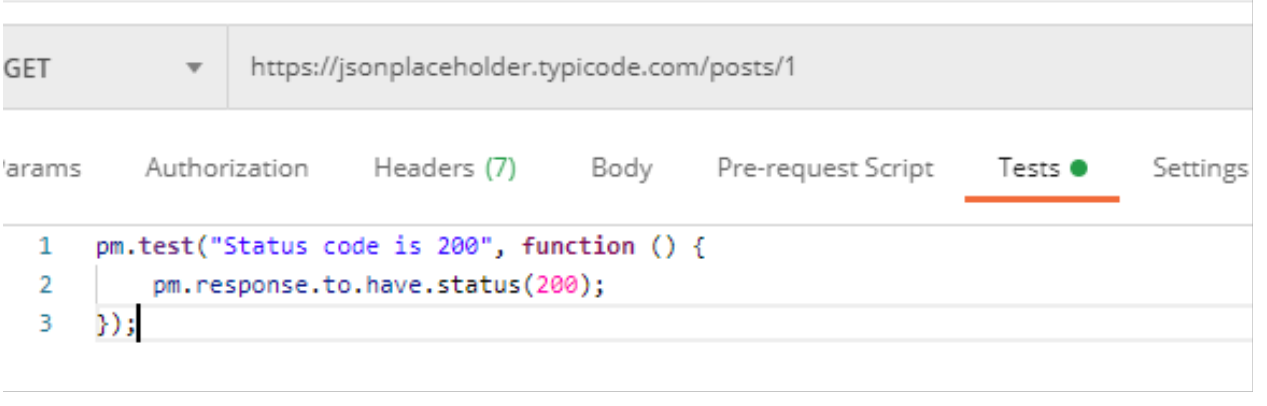
\includegraphics[width=8cm]{Imagenes/1}


2. En la parte derecha seleccionamos:

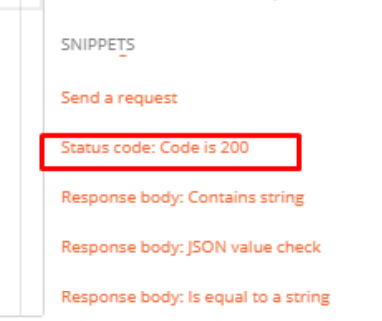
\includegraphics[width=8cm]{Imagenes/2}

3. Devolviendonos un JSON como resultado

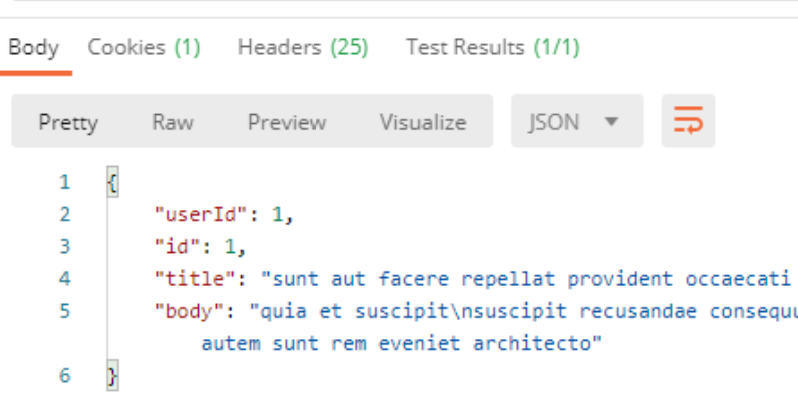
\includegraphics[width=8cm]{Imagenes/3}

4. Si nos dirigimos al aparto de test nos saldrá que el test tuvo exito.

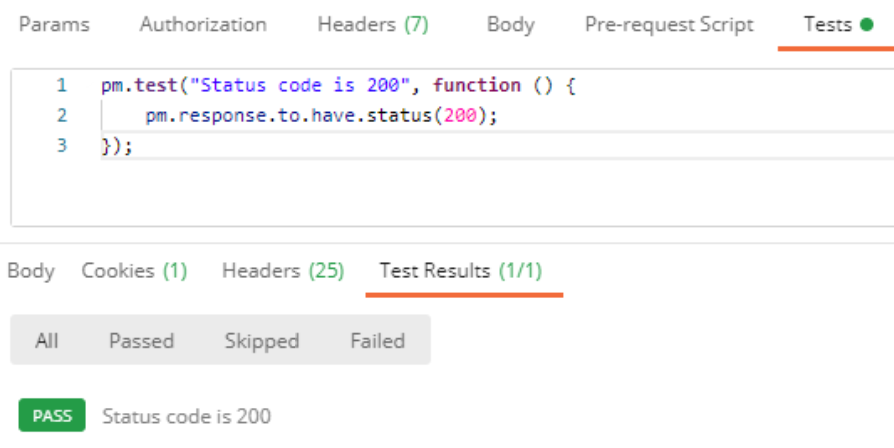
\includegraphics[width=8cm]{Imagenes/4}

5. En caso de que ingresemos una URL que no exista, en el test nos saldrá error.

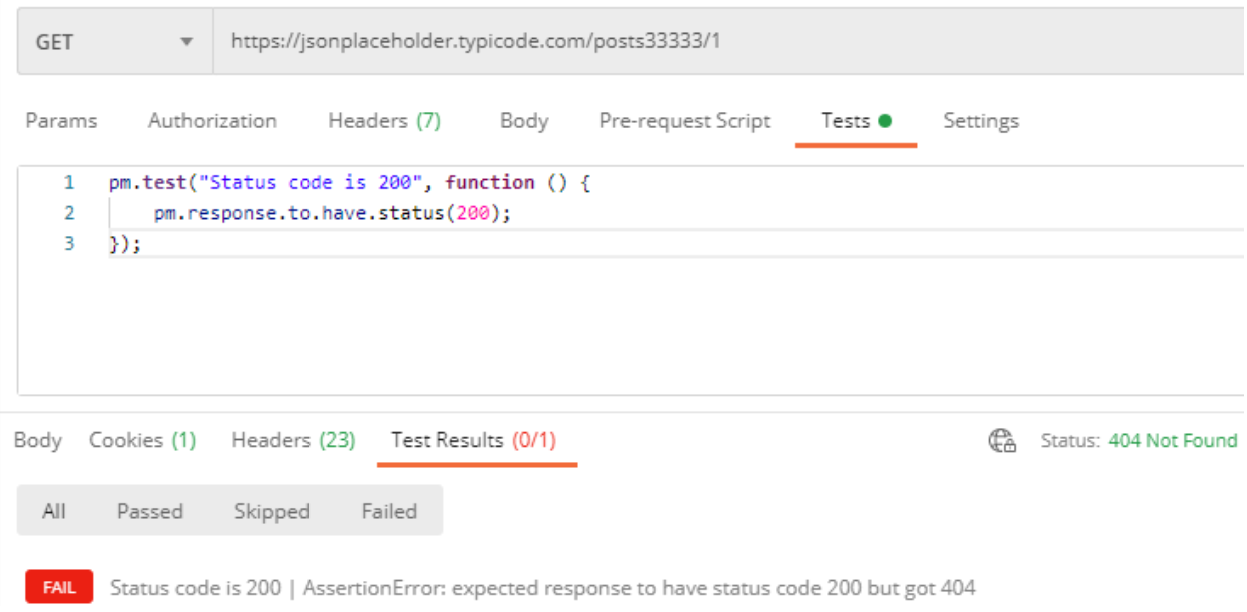
\includegraphics[width=8cm]{Imagenes/5}


%----------------------------------------------------------------------------------------
%	Conclusiones
%----------------------------------------------------------------------------------------


\section{Conclusiones}

Las pruebas automatizadas de API son fundamentales para la calidad del producto y los procesos de implementación continua CI y distribución continua CD. A diferencia de las pruebas de GUI, las pruebas de API pueden hacer frente a ciclos de lanzamiento cortos y cambios frecuentes, sin interrumpir los resultados de la prueba.

La prueba de API es una práctica de prueba de software que prueba las API directamente, desde su funcionalidad, confiabilidad, rendimiento y seguridad. Como parte de las pruebas de integración, las pruebas de API validan eficazmente la lógica de la arquitectura de compilación en un corto período de tiempo. 

Katalon Studio es una buena opción para pequeñas y medianas empresas. Es una solución en evolución con muchas integraciones que le permiten cubrir una variedad de tipos de pruebas con una sola herramienta. Viene con todas las instalaciones necesarias listas para usar para ejecutar varios tipos de pruebas, incluidas las pruebas de API. Es gratis y fácil de usar. Katalon puede ser utilizado por especialistas con diferentes roles de ingeniería de control de calidad y variadas habilidades de programación, lo que la convierte en una solución atractiva para equipos con probadores de diferentes niveles.

Postman es una herramienta que se utiliza, sobre todo, para el testing de API REST, aunque también admite otras funcionalidades que se salen de lo que engloba el testing de este tipo de sistemas. Postman nace como una herramienta que principalmente nos permite crear peticiones sobre APIs de una forma muy sencilla y poder, de esta manera, probar las APIs. Todo basado en una extensión de Google Chrome. El usuario de Postman puede ser un desarrollador que esté comprobando el funcionamiento de una API para desarrollar sobre ella o un operador el cual esté realizando tareas de mnonitorización sobre un API.

Alrededor de la idea de testear las APIs, Postman nos ofrece un conjunto de utilidades adicionales para poder gestionar las APIs de una forma más sencilla. Es por ello que nos va a proporcionar herramientas para documentar los APIs, realizar una monitorización sobre las APIs, crear equipos sobre un API para que trabajen de forma colaborativa.
%----------------------------------------------------------------------------------------
%	Recomendaciones
%----------------------------------------------------------------------------------------

\section{Recomendaciones}


\begin{itemize}
\item Presentadas estas opciones, si llega el momento de escoger una, quizá el mejor consejo es que antes de escribir esa primera línea de código para crear su propio framework, asegurarse de que no haya una biblioteca o framework existente que se pueda aprovechar, sería algo ilógico perder el tiempo reinventando la rueda; echar un vistazo a estos frameworks de automatización puede llegar a ser muy útil.
\item También se recomienda el uso de máquinas virtuales para evaluar con detenimiento cada uno de los frameworks y tener un panorama completo basado en pruebas específicas, luego se pueden presentar a un equipo de desarrollo sobre ordenadores reales.
\end{itemize}



%----------------------------------------------------------------------------------------
%	BIBLIOGRAFIA
%----------------------------------------------------------------------------------------

\selectlanguage{spanish}
\begin{thebibliography}{99} 

\bibitem[1]{}
\newblock Katalon LLC. (2019, 22 octubre). What is API Testing? | Definition, Benefits, Types \& Tool. Katalon Solution. https://www.katalon.com/api-testing/
\bibitem[2]{}
\newblock Editor. (2019, 9 diciembre). The Good and the Bad of Katalon Studio Automation Testing Tool. AltexSoft. https://www.altexsoft.com/blog/engineering/the-good-and-the-bad-of-katalon-studio-automation-testing-tool/
\bibitem[3]{}
\newblock HG Insights. (s. f.). Companies Using Katalon Studio, Market Share, Customers and Competitors. Recuperado 4 de diciembre de 2020, de https://discovery.hgdata.com/product/katalon-studio
\bibitem[4]{}
\newblock HG Insights. (s. f.-b). Companies Using Postman, Market Share, Customers and Competitors. Recuperado 4 de diciembre de 2020, de https://discovery.hgdata.com/product/postman
\bibitem[5]{}
\newblock Postman. (s. f.). Postman | The Collaboration Platform for API Development. Recuperado 4 de diciembre de 2020, de https://www.postman.com/
\bibitem[6]{}
\newblock Katalon. (2020, 1 diciembre). Katalon Trial and Free Plans. https://docs.katalon.com. https://docs.katalon.com/katalon-studio/docs/trial-free-plans.html
\bibitem[7]{}
\newblock Katalon LLC. (2020, 18 marzo). Katalon Pricing | Flexible Plans for Teams \& Projects of any size. Katalon Solution. https://www.katalon.com/pricing/
\bibitem[8]{}
\newblock Postman. (s. f.-a). Plans \& Pricing. Recuperado 4 de diciembre de 2020, de https://www.postman.com/pricing/
\bibitem[9]{}
\newblock Katalon Studio. (2020, 27 mayo). SoapUI vs Postman, Katalon Studio: A Review of Top 3 API Tools. Katalon Solution. https://www.katalon.com/resources-center/blog/soapui-vs-postman-katalon-api-tools/
\bibitem[10]{}
\newblock Du, H., Jones, P., Segarra, E. L., \& Bandera, C. F. (2018). Development of a REST API for obtaining site-specific historical and near-future weather data in EPW format.
\bibitem[11]{}
\newblock Soni, A., \& Ranga, V. (2019). API Features Individualizing of Web Services: REST and SOAP. International Journal of Innovative Technology and Exploring Engineering, 8, 664-671.
\bibitem[12]{}
\newblock Red Hat. (s. f.). ¿Qué es una API? Recuperado 5 de diciembre de 2020, de https://www.redhat.com/es/topics/api/what-are-application-programming-interfaces
\end{thebibliography}

%----------------------------------------------------------------------------------------


\end{document}
